\subsection{Configuration initiale (depuis la console)}
Une fois le serveur redémarré, il est nécessaire de lui attribuer ses adresses IP :
\begin{itemize}
    \item Choisir « 2 » pour assigner une adresse IP (figure \ref{fig:03-config-console-01})
    \item Choisir le numéro de l'adresse IP (figure \ref{fig:03-config-console-02})
    \item Choisir d'utiliser ou non DHCP (figure \ref{fig:03-config-console-03})
    \item Saisir l'adresse IP souhaitée (figure \ref{fig:03-config-console-04})
    \item Saisir le préfixe souhaité (figure \ref{fig:03-config-console-05})
    \item Saisir le masque désiré
    \item Ne pas définir de passerelle pour les réseaux locaux
    \item Procéder de la même manière pour l'IPv6
    \item Choisir d'activer le serveur DHCP ou non (figure \ref{fig:03-config-console-06})
    \item Ne pas activer le retour en http pour les connexions à l'interface d'administration (figure \ref{fig:03-config-console-07})
\end{itemize}

\begin{figure}[H]
    \centering
    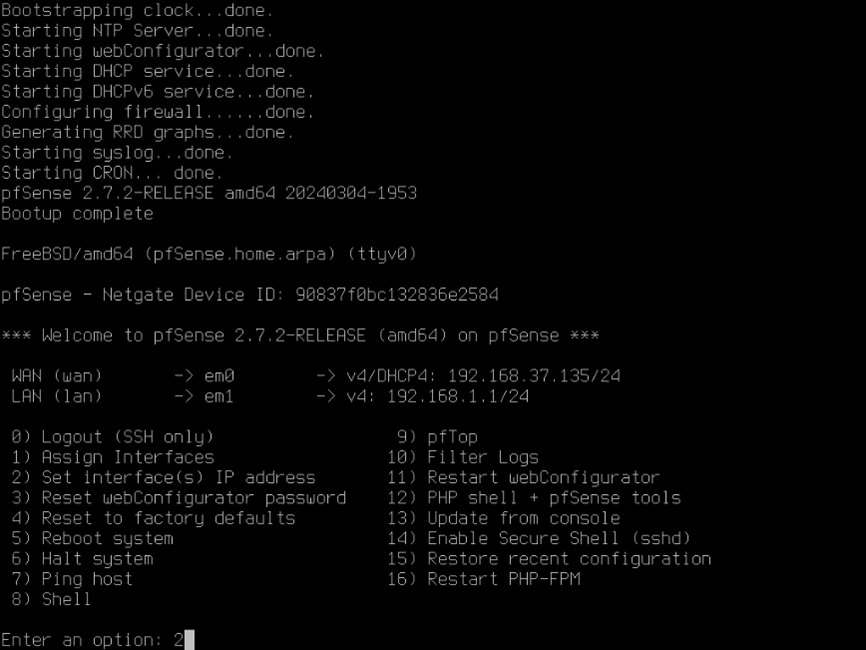
\includegraphics[width=0.88\textwidth]{03-Installation/Images/03-config-console-01.png}
    \caption{Configuration console - Choix de l'assignation d'adresses IP}
    \label{fig:03-config-console-01}
\end{figure}

\begin{figure}[H]
    \centering
    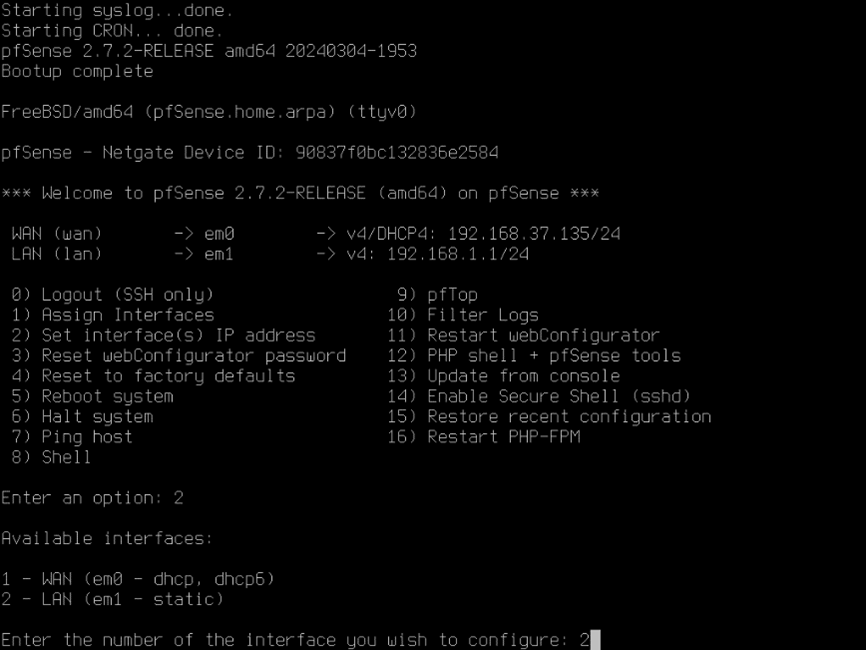
\includegraphics[width=0.88\textwidth]{03-Installation/Images/03-config-console-02.png}
    \caption{Configuration console - Choix de l'interface}
    \label{fig:03-config-console-02}
\end{figure}

\begin{figure}[H]
    \centering
    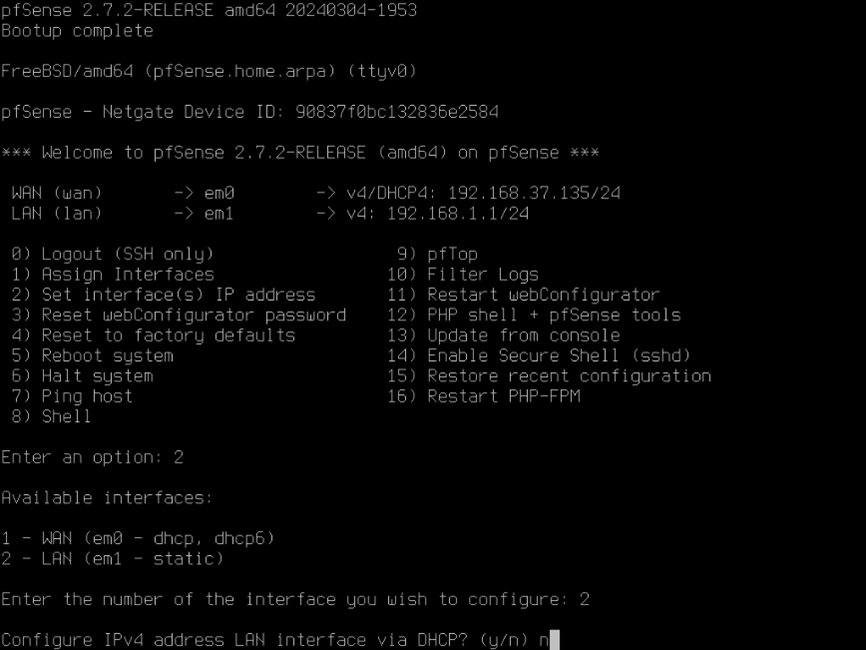
\includegraphics[width=0.88\textwidth]{03-Installation/Images/03-config-console-03.png}
    \caption{Configuration console - Choix de la non-utilisation de DHCP}
    \label{fig:03-config-console-03}
\end{figure}

\begin{figure}[H]
    \centering
    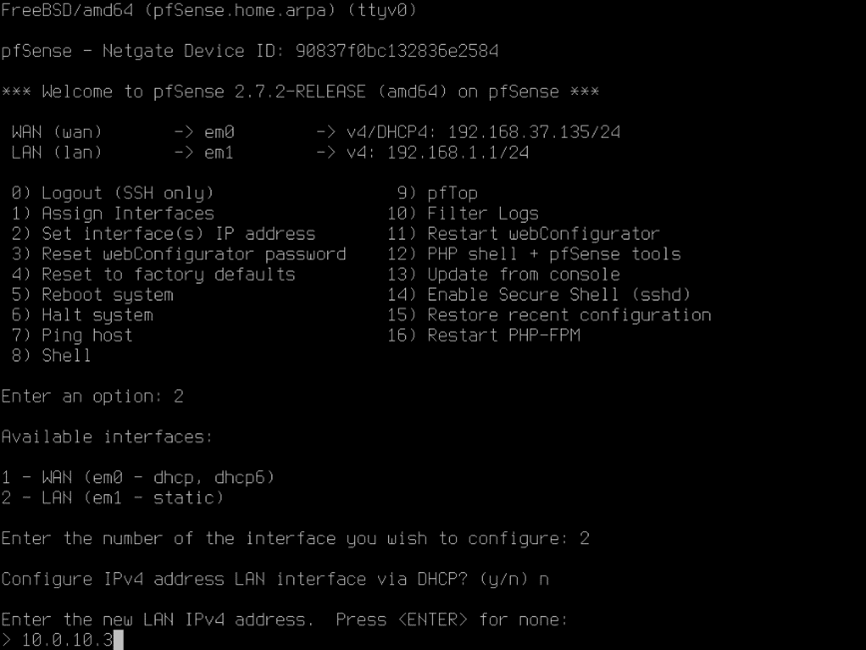
\includegraphics[width=0.88\textwidth]{03-Installation/Images/03-config-console-04.png}
    \caption{Configuration console - Définition de l'adresse IP}
    \label{fig:03-config-console-04}
\end{figure}

\begin{figure}[H]
    \centering
    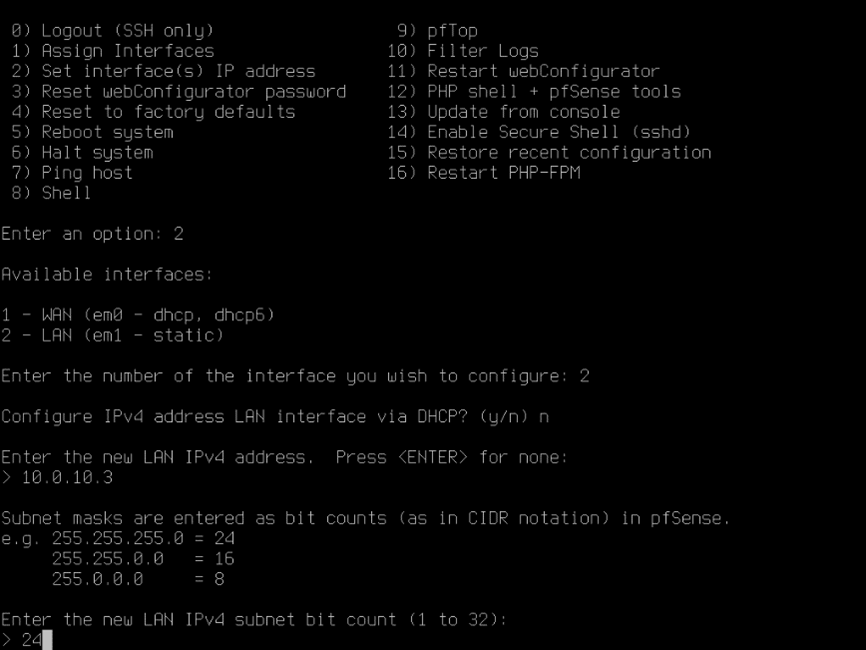
\includegraphics[width=0.88\textwidth]{03-Installation/Images/03-config-console-05.png}
    \caption{Configuration console - Définition du préfixe}
    \label{fig:03-config-console-05}
\end{figure}

\begin{figure}[H]
    \centering
    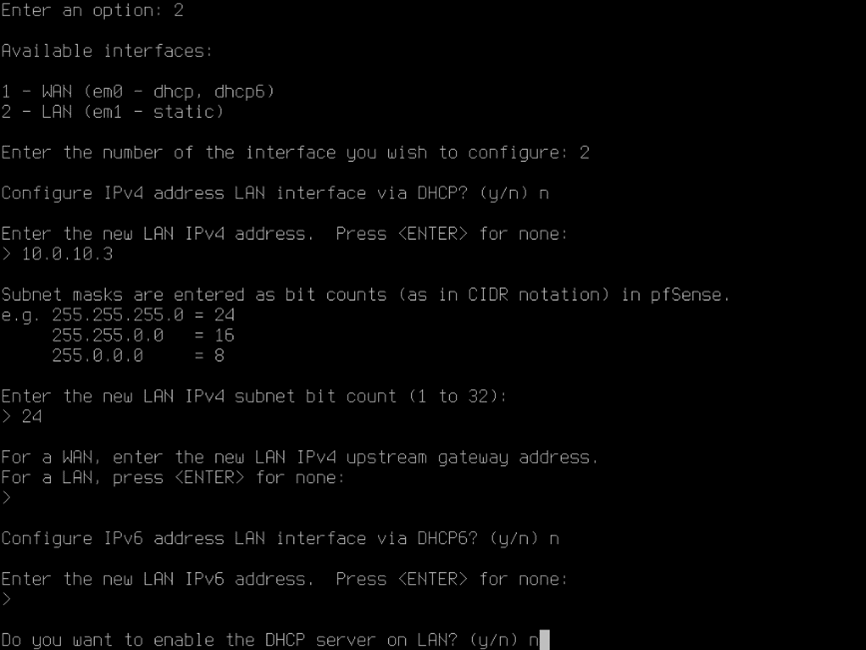
\includegraphics[width=0.88\textwidth]{03-Installation/Images/03-config-console-06.png}
    \caption{Configuration console - Non-activation du serveur DHCP}
    \label{fig:03-config-console-06}
\end{figure}

\begin{figure}[H]
    \centering
    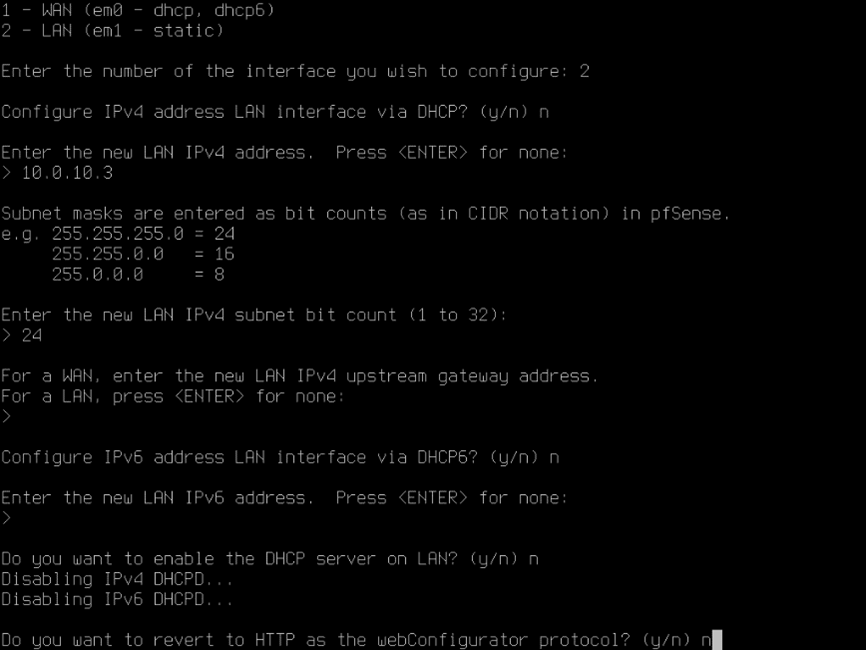
\includegraphics[width=0.88\textwidth]{03-Installation/Images/03-config-console-07.png}
    \caption{Configuration console - Non-activation du retour HTTP}
    \label{fig:03-config-console-07}
\end{figure}